\section{Pressure}
The thermodynamic pressure is caused by particles colliding with a wall and
hence exerting a force on that wall. By a potential energy analysis, it has been
shown that we can compute the pressure using the PCF according
to \cite{ravndal:statPhys}
\begin{equation}
	\frac{\beta P}{\rho} = 1 - \frac{\rho}{6k_B T} \int d^3r r u'(r) g(r).
\end{equation}

To determine the error in the pressure measurement, it is required to determine
the `correlation time'. This is a characteristic time we need to wait between
two measurements to be able to call those measurements independent. The
autocorrelation function for the solid2 case is shown in
\figref{fig:autocorr_pressure}.
Judging from this autocorrelation function (note the y-scale!), I would
conclude that each and every measurement is effectively independent.
Also, if we compute $<P^2>$ and $<P>^2$, I find the very same number
up to four significant digits.
However, it makes little sense that the system is independent after a timestep
of $O(10^{-3})$. I cannot figure out what is wrong, so, I would like to dare the
reader to explain this autocorrelation function. In principle, the maximum
should \textbf{always} occur at $\tau = 0$, but it does not. And worst of all:
``numerical error'' cannot explain it.

\begin{figure}
	\centering
	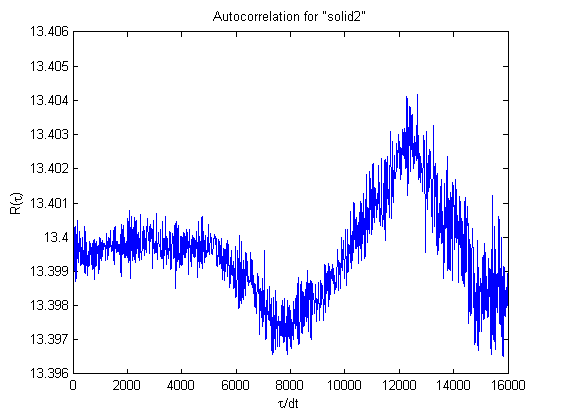
\includegraphics[width=0.5\textwidth]{../Graphs/Autocorrelation_solid2.png}
	\caption{Autocorrelation function for the solid2 case.}
	\label{fig:autocorr_pressure}
\end{figure}

Nonetheless, if we assume that the system is independent after 1000 iterations,
we can still compute the standard deviation based on that assumption.
A summary of these results are given in \tabref{tab:pressure}, together with
Verlet's \cite{verlet:firstPaper} value for similar cases. We see that our
simulations are in accordance with Verlet's results.

As a further validation, the gas2 case was performed for a reason: it models
Argon at 0$\cels$ at atmospheric pressure. I have inserted the density of Argon
and the given temperature and computed the pressure. This resulted in $1.0125
\pm 2\cdot 10^{-5}$ bar with a mean temperature of $272.9K$, which is extremely
close to the value $1.01325$ bar. If we accept the ideal gas law, we note that
$T \propto P$. So, if we compensate our mean temperature with a factor
$\frac{273.15 K}{272.9 K}$, we should have a more accurate result. This results
in $1.0134$ bar. This is a strong indication that my pressure calculation is
correct.

\begin{table}
\centering
\caption{Pressure for several test cases. The standard deviation for each
measurement is $O(3 \cdot 10^{-3})$.} \begin{tabular}{|c|c|c|c|c|} \hline
$\rho$&$T_{me}$&$T_{Verlet}$&$(\beta P/\rho)_{me}$&$(\beta P/\rho)_{Verlet}$ \\
\hline
0.88&0.945&0.94&2.78&2.72\\ \hline
0.85&1.119&1.128&2.69&2.78\\ \hline
0.75&0.889&0.881&-0.12&-0.12\\ \hline
0.65&2.546&2.557&2.11&2.14\\ \hline
0.45&1.754&1.744&0.75&0.74\\ \hline
0.45&1.548&1.552&0.53&0.75\\ \hline
0.35&1.433&1.418&0.39&0.40\\ \hline
\end{tabular}
\label{tab:pressure}
\end{table}

Note that a negative pressure implies that the particles are `imploding' due to
their mutual interactions: there is a strong tendency to be pulled together,
rather than being confined by the environment. This is typical for a solid.

